\chapter{Open Source Anonymous Credentials Benchmark Library}\label{chap6}
Anonymous Credentials lack a standardized, practical evaluation tool which will hinder adoption progress. I introduce an open-source library in Rust that benchmarks state-of-the-art Attribute-Based Anonymous Credential (ABC) schemes under consistent conditions. The field suffers from inconsistent comparisons—varying languages (e.g., Python, C++, Rust) and libraries (e.g., Arkworks, Ethereum PyEcc)—making it hard to assess schemes like BBS+ and PS fairly. Our work bridges this gap, offering practitioners a tool to understand functional differences and performance trade-offs while revealing how cryptographic optimizations enhance efficiency beyond theoretical predictions.

\section{Core Contributions}
My primary contribution is an open-source Rust library that implements and benchmarks leading ABC schemes (e.g., BBS+, PS, and their variants), providing a standardized framework for fair comparisons. Unlike prior evaluations, which lack consistency, our library ensures identical conditions—same hardware, security parameters, and libraries—highlighting the most efficient scheme for the critical ``Show + Verify'' operation (e.g., PS-UTT22 at 5.38 ms for 30 attributes, a 6.09x speedup over PS16). This tool also serves as an educational resource, helping practitioners explore constructions and select schemes for use cases like decentralized identity or Sybil-resistant voting.

My second contribution demonstrates the gap between theoretical and practical cryptography through the empirical evaluation of two optimizations:
\begin{enumerate}
    \item \textbf{Schnorr Proofs with Multi-Scalar Multiplication (MSM):} I show that Schnorr proofs, often criticized as linear in attribute size, scale sublinearly in practice using MSM, challenging theoretical assumptions and boosting efficiency in New Generation Anonymous Credential schemes using $\G_1$ Schnorr proofs.
    
    \item \textbf{Pairing Optimizations Pairings:} By leveraging Miller-Loop optimizations, I show pairing computation cost can be reduced,  improving pairing-based credential performance.
\end{enumerate}

These findings, validated in our library, extend beyond ABCs, offering insights for broader cryptographic applications.



\section{Fair Anonymous Credential Microbenchmarks}

The results table \ref{abc-performance-combined-table-chap6} demonstrates the standardized benchmark results from my Anonymous Credential library \cite{polgar_anonymous_2025}, demonstrating newer anonymous credential schemes, such as BBS+2016 \cite{camenisch_anonymous_2016} and PS-UTT22 \cite{tomescu_utt_2022}, outperform older schemes like BBS+06 \cite{hutchison_constant-size_2006} and PS16 \cite{sako_short_2016} by shifting zero-knowledge proofs from the target group $(\mathbb{G}_T)$ to the source group ($\mathbb{G}_1)$\footnote{\cite{hutchison_signature_2004} is included in previous generation}. For 30 attributes, older schemes require computing over 3$\ell$, and 2$\ell$ $\G_T$ points respectively with Show and Verify times of 39.21 ms (BBS+06) and 32.78 ms (PS16). In comparison, newer schemes compute only in $\G_1$ and minimize pairings, achieving times of 5.72 ms and 5.38 ms—speedups of 6.85x and 6.09x, respectively. These improvements maintain full functionality, including selective disclosure and unlinkability, and rely on standard security assumptions, enhancing the practicality of anonymous credentials for digital identity systems.



\begin{table}[!htbp]
\centering
\caption{Performance Comparison of Anonymous Credential Schemes for Show and Verify Algorithms ($\ell = 30$ Attributes)}
\label{tab:anon_creds_performance_old_gen_vs_new}
\begin{tabular}{|l|c|c|c|c|c|c|}
\hline
\textbf{Scheme} & \textbf{ZKPoK}  & \textbf{Show (ms)} & \textbf{Verify (ms)}  & \textbf{Show + Verify (ms)} & \textbf{Speedup} \\
\hline
BBS+06 & $\mathbb{G}_T$ & 12.91  & 26.30 & 39.21 & -- \\
\hline
BBS+2016 & $\mathbb{G}_1$ & 3.15  & 2.57 & 5.72 & 6.85x over BBS+ 06 \\
\hline
PS16 & $\mathbb{G}_T$ & 16.23  & 16.55 & 32.78 & -- \\
\hline
PS-UTT22 & $\mathbb{G}_1$ & 1.59  & 3.79 & 5.38 & 6.09x over PS16 \\
\hline
\end{tabular}
\end{table}












\section{Evaluating Cryptography Library Optimizations}
A key challenge when assessing Anonymous Credential constructions is the use of optimizations lowering computational cost and therefore making practical benchmarks unclear and potentially unfair comparisons between different libraries. Optimizations like Multi-Scalar Multiplication and Pairing techniques lower computational cost. 
Below, I explore the impact of these optimizations: 



\subsection{Schnorr Proofs with Multi-Scalar Multiplication (MSM) are Sublinear}\label{sigma-protocol-analysis}

$\Sigma$-protocols, such as Schnorr proofs, are often characterized as having linear complexity with respect to the number of attributes. However, by leveraging multi-scalar multiplication (MSM)—an optimized algorithm widely available in cryptographic libraries—we demonstrate that these proofs achieve sublinear scaling in practice. MSM efficiently computes sums of scalar multiplications in elliptic curve groups, reducing the computational cost of proof generation and verification compared to naive approaches. This positively impacts the performance of Anonymous Credential schemes that leverage $\Sigma$-protocols. Figure \ref{fig:schnorr-benchmarks} provides benchmark results, illustrating the sublinear scaling as the number of attributes increases.

\begin{figure}[!htb]
    \centering
    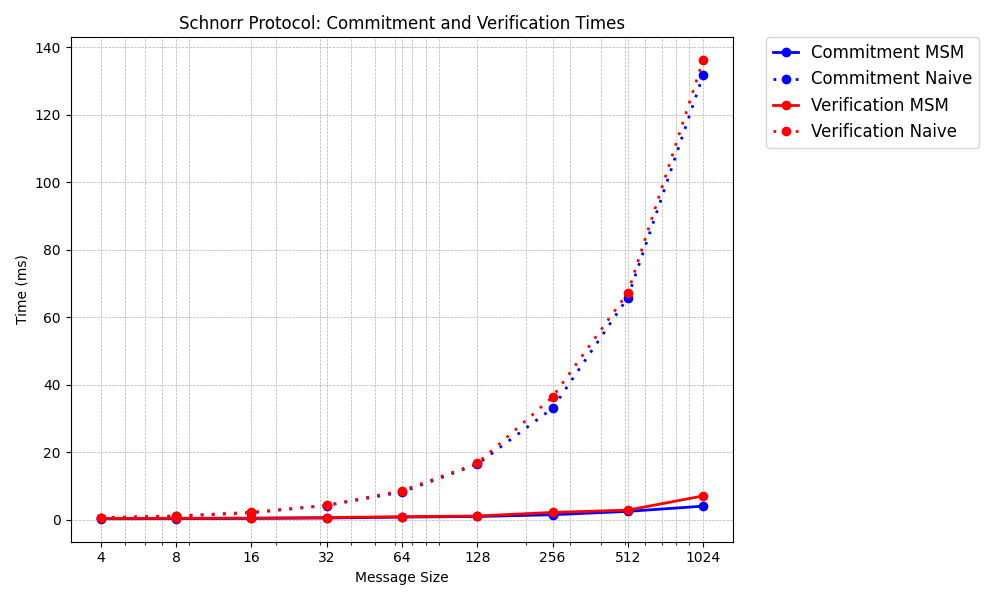
\includegraphics[width=0.75\linewidth]{schnorr_msm_no_msm.png}
    \caption{Schnorr Protocol - Practical Benchmarks with Multi-Scalar Multiplication}
    \label{fig:schnorr-benchmarks}
\end{figure}





\subsection{Optimizations for Pairing Protocols }

Pairing-based cryptography underpins many anonymous credential schemes, enabling functionalities like zero-knowledge proofs and attribute-based signatures through bilinear maps. However, pairings are computationally expensive, often dominating the runtime of schemes such as BBS+06~\cite{hutchison_constant-size_2006} and PS16~\cite{sako_short_2016}. Most theoretical analyses, such as those in~\cite{sako_short_2016}, measure complexity as a count of pairing operations (e.g., $3\ell$ or $2\ell$ pairings for $\ell$ attributes), overlooking practical optimizations available in modern cryptographic libraries. In this subsection, we detail two key optimizations—Miller Loop with Final Exponentiation and Batch Pairing Inversion—implemented in our open-source Rust library, and demonstrate their impact on bridging the gap between theoretical complexity and practical performance.

\subsubsection*{Miller Loop and Final Exponentiation}
A pairing operation, such as the Tate or Ate pairing, denoted $e(P, Q)$, comprises two phases: the Miller Loop, which computes a rational function over elliptic curve points, and the Final Exponentiation, which maps the result to a unique element in the target group $\mathbb{G}_T$. For a product of $\ell$ pairings:
\[
\prod_{i=1}^\ell e(g_i, \hat{h}_i),
\]
a naive implementation computes $\ell$ full pairings, each requiring a Miller Loop and a Final Exponentiation, followed by $(\ell-1)$ multiplications in $\mathbb{G}_T$. This incurs a cost of approximately $\ell P + (\ell-1)M_{\mathbb{G}_T}$, where $P$ is the cost of one pairing and $M_{\mathbb{G}_T}$ is a multiplication in $\mathbb{G}_T$. However, by exploiting bilinearity, we optimize this as:
\[
\prod_{i=1}^\ell e(g_i, \hat{h}_i) = \text{FinalExp}\left( \prod_{i=1}^\ell \text{MillerLoop}(g_i, \hat{h}_i) \right).
\]
Here, the computation reduces to $\ell$ Miller Loops (each roughly 40\% of a pairing’s cost, or $0.4\ell P$) and one Final Exponentiation (approximately 60\% of a pairing, or $0.6P$), eliminating the need for additional $\mathbb{G}_T$ multiplications. For large $\ell$, this yields significant savings, as the single Final Exponentiation amortizes across all pairings.


\begin{figure}
    \centering
    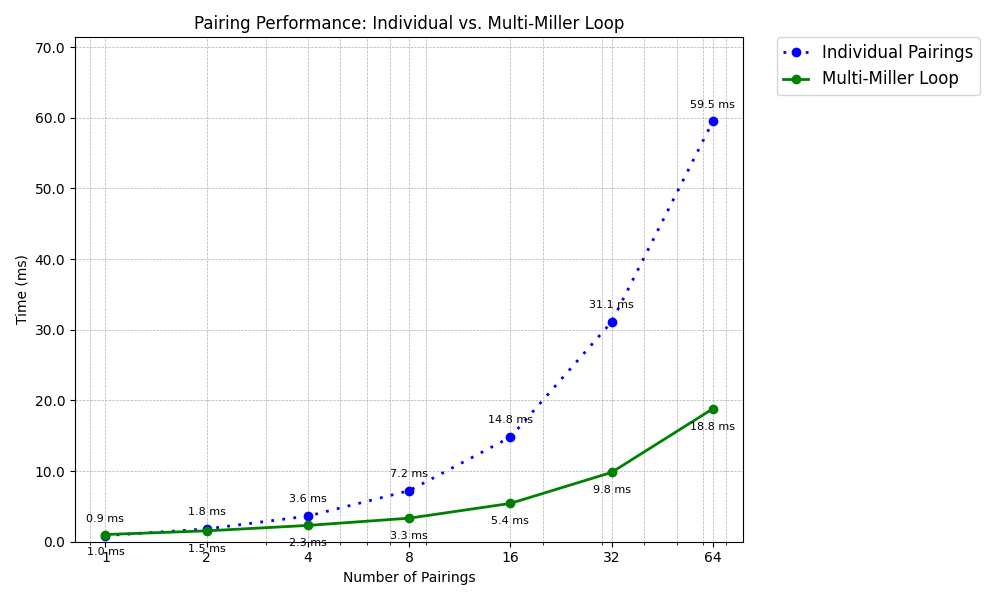
\includegraphics[width=0.75\linewidth]{pairing_comparison.png}
        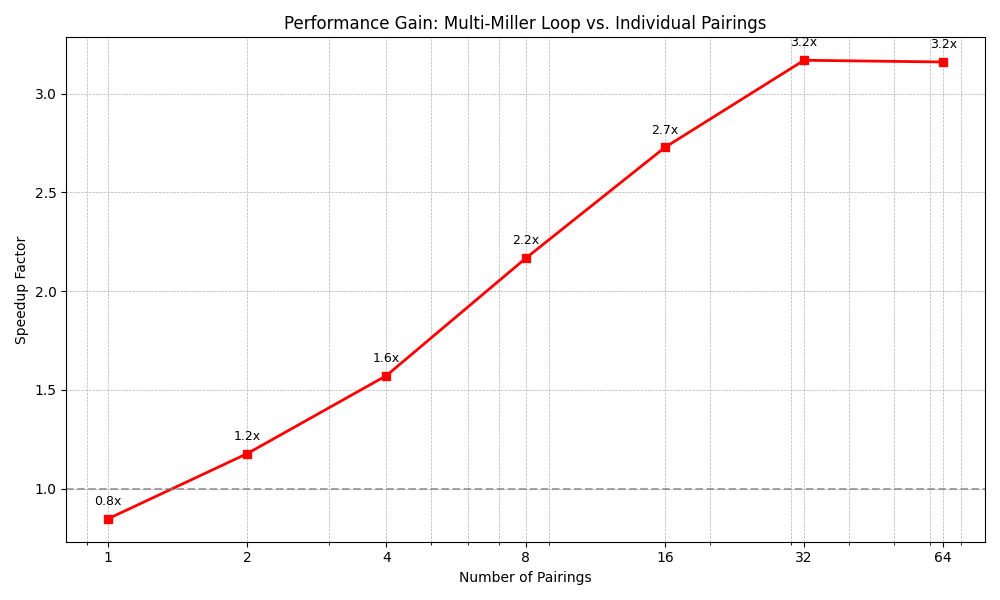
\includegraphics[width=0.75\linewidth]{pairing_comparison2.png}
    \caption{Elliptic Curve Pairings - Practical Benchmarks with Miller-Loop Intermediate Computation}
    \label{fig:elliptic_curve_pairings_speedup}
\end{figure}



\subsubsection*{Batch Pairing Inversion}
Verification of pairing equalities, such as $e(a, b) = e(c, d)$, is common in credential schemes. Naively, this requires two full pairing computations and a comparison in $\mathbb{G}_T$. Batch Pairing Inversion transforms this into a single check:
\[
e(a, b) \cdot e(c^{-1}, d) \stackrel{?}{=} 1_{\mathbb{G}_T},
\]
where $c^{-1}$ is the inverse of $c$ in its source group. By combining the pairings into a product, this reduces the cost from two standalone pairings (approximately $2P$) to one optimized pairing (approximately $P$), cutting computation time by nearly 50\% in multi-equality scenarios, such as verifying credentials with multiple attributes.

% Connecting optimizations to practical performance
\subsubsection*{Practical Impact}
These optimizations, implemented in our Rust library using frameworks like Arkworks, significantly enhance the performance of pairing-based anonymous credentials. For instance, older schemes like PS16 and BBS+06, which rely heavily on $\mathbb{G}_T$ operations, see verification times of 32.78~ms and 39.21~ms for 30 attributes (Table~\ref{tab:anon_creds_performance_old_gen_vs_new}). By applying Miller Loop and Final Exponentiation optimizations, we reduce the pairing overhead, while Batch Pairing Inversion streamlines equality checks in verification. Benchmarks, visualized in Figure~\ref{fig:elliptic_curve_pairings_speedup}, show that these techniques yield speedups of up to 2x for pairing-intensive operations compared to unoptimized implementations. When combined with the shift to $\mathbb{G}_1$-based proofs in newer schemes like PS-UTT22 and BBS+2016, the cumulative effect is a 6x performance boost, underscoring the critical role of practical optimizations.



\section{Impact and Conclusion}

My work addresses the challenge of inconsistent ABC evaluations by delivering a standardized Rust-based benchmarking library. Through rigorous empirical analysis, I uncover performance improvements as sent throughout the Thesis. These results bridge the divide between theoretical cryptography and real-world implementation, facilitating the adoption of ABCs in applications such as decentralized identity and secure voting systems. While currently focused on Rust-compatible schemes, future enhancements could integrate additional cryptographic primitives and optimizations, broadening its scope. Ultimately, this library empowers the cryptographic community with a resource for learning and implementing privacy-preserving technologies.




\begin{table}[htbp]\label{abc-performance-combined-table-chap6}
\centering
\caption{Performance of Anonymous Credential Operations (time in ms), $n$ is attribute count}
\begin{tabular}{@{}p{1.2cm}*{5}{>{\centering\arraybackslash}p{1.6cm}}@{}}
\toprule
$n$ & \cite{hutchison_constant-size_2006} & \cite{camenisch_anonymous_2016} & \cite{sako_short_2016} & \cite{tomescu_utt_2022} \ref{sec:formal_treatment_utt_rerand_sig} & Our Improved \ref{sec:formal_treatment_utt_rerand_sig} \\
\midrule
\multicolumn{6}{c}{\textbf{Obtain}}  \\
\midrule
\textbf{2} & 0.51 & 0.90 & 0.66 & 0.25 & \textbf{0.23} \\
\textbf{5} & 0.65 & 1.00 & 0.66 & 0.28 & \textbf{0.27} \\
\textbf{10} & 0.67 & 1.13 & 0.82 & 0.36 & \textbf{0.31} \\
\textbf{15} & 0.78 & 1.26 & 0.87 & 0.37 & \textbf{0.36} \\
\textbf{20} & 0.86 & 1.38 & 0.94 & \textbf{0.41} & \textbf{0.41} \\
\textbf{30} & 1.07 & 1.63 & 1.11 & 0.51 & \textbf{0.49} \\
\midrule
\multicolumn{6}{c}{\textbf{Issue}}  \\
\midrule
\textbf{2} & 1.25 & \textbf{0.72} & 1.48 & 1.27 & 2.99 \\
\textbf{5} & 1.66 & \textbf{0.75} & 1.79 & 1.66 & 3.31 \\
\textbf{10} & 2.33 & \textbf{0.83} & 2.54 & 2.35 & 4.00 \\
\textbf{15} & 2.98 & \textbf{0.84} & 3.23 & 3.03 & 4.64 \\
\textbf{20} & 3.96 & \textbf{0.90} & 3.79 & 3.66 & 5.88 \\
\textbf{30} & 4.97 & \textbf{0.94} & 5.16 & 5.10 & 6.86 \\
\midrule
\multicolumn{6}{c}{\textbf{Show}}  \\
\midrule
\textbf{2} & 5.39 & 2.31 & 3.20 & \textbf{1.14} & 1.29 \\
\textbf{5} & 6.05 & 2.42 & 3.15 & \textbf{1.16} & 1.29 \\
\textbf{10} & 7.44 & 1.71 & 4.53 & \textbf{1.22} & 1.33 \\
\textbf{15} & 8.86 & 2.71 & 6.14 & 1.40 & \textbf{1.37} \\
\textbf{20} & 11.88 & 1.88 & 7.66 & \textbf{1.41} & 1.51 \\
\textbf{30} & 12.91 & 3.15 & 16.23 & \textbf{1.37} & 1.59 \\
\midrule
\multicolumn{6}{c}{\textbf{Verify}}  \\
\midrule
\textbf{2} & 7.59 & 2.18 & 4.57 & 2.47 & \textbf{1.79} \\
\textbf{5} & 9.25 & 2.25 & 5.52 & 2.73 & \textbf{2.01} \\
\textbf{10} & 11.09 & \textbf{2.25} & 7.10 & 3.16 & 2.44 \\
\textbf{15} & 13.96 & \textbf{2.30} & 8.62 & 3.47 & 2.72 \\
\textbf{20} & 16.93 & \textbf{2.34} & 9.88 & 3.84 & 3.21 \\
\textbf{30} & 26.30 & \textbf{2.57} & 16.55 & 4.67 & 3.79 \\
\midrule
\multicolumn{6}{c}{\textbf{Issuing Phase Total (Obtain + Issue)}}  \\
\midrule
\textbf{2} & 1.76 & 1.62 & 2.14 & \textbf{1.53} & 3.22 \\
\textbf{5} & 2.31 & \textbf{1.76} & 2.45 & 1.95 & 3.57 \\
\textbf{10} & 3.00 & \textbf{1.96} & 3.37 & 2.71 & 4.31 \\
\textbf{15} & 3.75 & \textbf{2.10} & 4.10 & 3.40 & 5.00 \\
\textbf{20} & 4.82 & \textbf{2.29} & 4.74 & 4.06 & 6.28 \\
\textbf{30} & 6.04 & \textbf{2.57} & 6.27 & 5.60 & 7.35 \\
\midrule
\multicolumn{6}{c}{\textbf{Showing Phase Total (Show + Verify)}}  \\
\midrule
\textbf{2} & 12.98 & 4.48 & 7.77 & 3.61 & \textbf{3.08} \\
\textbf{5} & 15.30 & 4.67 & 8.68 & 3.90 & \textbf{3.30} \\
\textbf{10} & 18.53 & 3.96 & 11.62 & 4.38 & \textbf{3.77} \\
\textbf{15} & 22.82 & 4.22 & 14.76 & 4.87 & \textbf{4.09} \\
\textbf{20} & 28.81 & 5.01 & 17.53 & 5.25 & \textbf{4.72} \\
\textbf{30} & 39.21 & 5.72 & 32.77 & 6.04 & \textbf{5.37} \\
\bottomrule
\end{tabular}
\end{table}

\clearpage